% \begin{frame}
%     \frametitle{Nash Equilibrium}
%     \centering

%     \scriptsize
%     \begin{equation*}
%         R =  
%         \begin{pmatrix}
%             0.5 & 0.1 & 0 & 0 \\
%             0.9 & 0.5 & 0.2 & 0 \\
%             1 & 0.8 & 0.5 & 0.3 \\
%             1 & 1 & 0.7 & 0.5
%         \end{pmatrix}
%     \end{equation*}
%     \begin{equation*}
%         A = 
%         \begin{pmatrix}
%             8.39 & 8.39 & 8.39 & 8.39 \\
%             8.96 & 8.85 & 8.65 & 8.45 \\
%             9.95 & 9.87 & 9.6  & 9.2  \\
%             4.37 & 5.11 & 8.6  & 9.91 \\
%         \end{pmatrix}
%     \end{equation*}
%     \begin{equation*}
%         B = 
%         \begin{pmatrix}
%             8.39 & 8.96 & 9.95 & 4.37 \\
%             8.39 & 8.85 & 9.87 & 5.11 \\
%             8.39 & 8.65 & 9.6 &  8.6 \\ 
%             8.39 & 8.45 & 9.2 &  9.91 \\
%         \end{pmatrix}
%     \end{equation*}

%     \begin{equation*}
%         \textbf{Nash Equilibria: } 
%         \begin{array}{cc}
%             \underline{\quad A \quad} & \underline{\quad B \quad} \\
%             % (0, 0, 1, 0) & (0, 0, 1, 0) \\ 
%             % (0, 0, 0, 1) & (0, 0, 0, 1) \\ 
%             (0, 0, 0.4, 0.6) & (0, 0, 0.4, 0.6) 
%         \end{array}
%     \end{equation*}
% \end{frame}


\begin{frame}
    \frametitle{Asymmetric Replicator Dynamics}
    \centering

    \[
        \frac{dx}{dt}_i = x_i((f_x)_i - \phi_x), \quad \text{ for all }i
    \]
    \[
        \frac{dy}{dt}_i = y_i((f_y)_i - \phi_y), \quad \text{ for all }i
    \]
    
\end{frame}


% \begin{frame}
%     \frametitle{Inefficiency measure}

%     \begin{equation*}
%         PoA = \frac{\max_{s \in E} Cost(s)}{\min_{s \in S} Cost(S)}
%     \end{equation*}
%     \pause
%     \footnotesize
%     \vspace{1cm}
%     \begin{equation*}
%         PoA_A(s_r) = \frac{Cost(s_r)}{\min_{s \in S} Cost(S)}, \hspace{1cm} 
%         PoA_B(s_c) = \frac{Cost(s_c)}{\min_{s \in S} Cost(S)}
%     \end{equation*}
% \end{frame}


\begin{frame}
    \frametitle{Learning algorithms - Asymmetric replicator dynamics}

    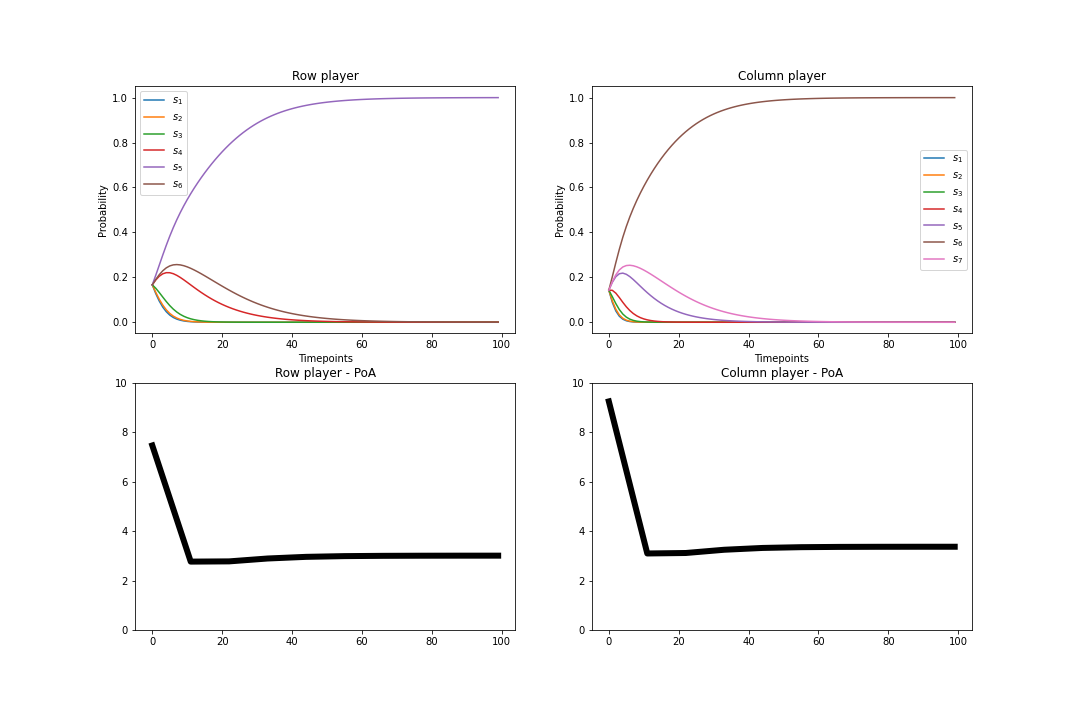
\includegraphics[scale=0.28]{Bin/ARD_game.png}
\end{frame}

\begin{frame}
    \centering
    \Huge{
    Inefficiencies can be learned and emerge naturally
    }
\end{frame}


\begin{frame}
    \frametitle{Learning algorithms - Asymmetric replicator dynamics}

    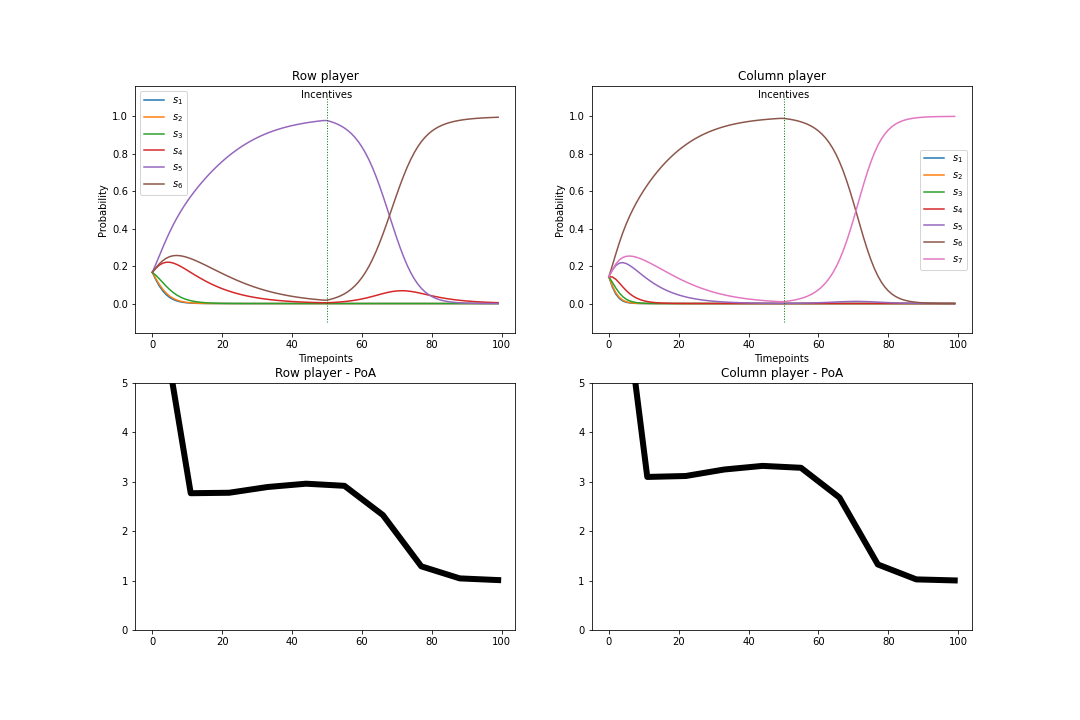
\includegraphics[scale=0.28]{Bin/ARD_penalty_game.png}
    
\end{frame}


\begin{frame}
    \centering
    \Huge{
    Targeted incentivisation of behaviours can help escape learned inefficiencies
    }
\end{frame}
